%!TEX root = ../thesis.tex
%*******************************************************************************
%*********************************** First Chapter *****************************
%*******************************************************************************

\chapter{Semiconductors and Diamond}

\ifpdf
    \graphicspath{{Chapter1/Figs/Raster/}{Chapter1/Figs/PDF/}{Chapter1/Figs/}}
\else
    \graphicspath{{Chapter1/Figs/Vector/}{Chapter1/Figs/}}
\fi


\label{ch:semiconductors_and_diamond}
%bbc article. Very accessible reading and trying to paint a picture of where dimaond fits in as an electronic material in a way that makes sense without stuff like definitions of electron affinity... unless I can make that understandable I guess...

\section{The Development of Electrical Devices}
\subsection{A Brief History of Electricity}
Electricity has been a known phenomena for thousands of years. Ancient Egyptian texts from 2750 BCE refer to a "thunderer of the Nile" as the protector of fish, now known as the electric catfish Malapterurus electricus \cite{moller1991}. Perhaps the next step in the timeline of electricity is the discovery in 585 BCE by Thales of Miletus that rubbing certain objects (such as amber or fur) together would cause an attraction of other nearby objects. This is now known to be "static" electricity. At the start of the seventeeth century, William Gilbert published his book (De Magnete) on magnetism, including arguments a that his experiments proved the earth had a magnetic field and that the Earth rotated on its axis \cite{gilbert1600}. This became one of the most controversial works of its time, with multiple reprints and condemnation during the trial of Galileo in 1633 \cite{linder2002}. This book contained the first usage of "electric" in the form "electricus" as a variation on the Greek word for amber "elektron".

In 1730 the terms conductor and insulator were used for the first time by Stephen Gray \cite{carnle1931}, which was later famously followed by the first usage of 'negative' and 'positive' in Benjamin Franklin's 1751 work, during which he sold his possessions as a source of funding and proved that lightning was caused by static electricity \cite{park1898} \cite{uman1986}. 

Next, in 1780 Luigi Galvani found that when a frog was touched by an electrical spark, its legs would twitch \cite{whittaker1953}. Alessandro Volta was then one of the first to repeat and confirm these experiments, with the added observation that the metal wires used would impact the resulting muscle contractions. This was shortly followed by Volta's alternating zinc and copper battery, also known as the voltaic pile \cite{guarnieri2014}. In 1820, Hans {\O}rsted established that electricity and magnetism were linked, with an electric current passing through a wire generating a magnetic field, displacing the needle of a compass. Subsequent to this in 1821, Michael Faraday discovered that the inverse was also true, that of a magnetic field generating an electric field. Since the movement of magnets and electric charges was now linked, this could be exploited to create an electric motor. In 1826 Andr{\'e}-Marie Amp{\'e}re found the magnetic field strength that attracts two current carrying wires together. A year later, George Ohm published a complete mathematical theory of electricity, with the unit of electrical resistance named after him (Ohms). The principles of an electrical generator (a dynamo) were discovered in 1830 by Joseph Henry. In 1831 Michael Faraday demonstrated the principle of electromagnetic induction with a magnet passing through a coiled wire. The velocity of electricity was successfully measured in 1834 by Charles Wheatstone, with an experiment comprising a rotating mirror and four miles of wire. Samuel Morse invented Morse Code, with a demonstration of 10 transmitted words per minute in 1838 via the telegraph machine.

One of the most influential authors from the 19th century was that of James Clerk Maxwell. His first contribution was to generalise the work of Amp{\'e}re to fully define the forces due to a moving electronic charge in 1855 \cite{maxwell1890}. Then, with a four-part paper in 1861, he established the four laws of electromagnetism \cite{maxwell2010}. The magnitude of these laws (commonly known as Maxwell's equations) places Maxwell among some of the most lauded of physicists or indeed scientists as a whole, such as Isaac Newton and Albert Einstein.

As the 19th century progressed, vacuum tubes were used to reveal the presence of the electron as a fundamental charge carrying particle. These tubes started out as "Geissler tubes", the precurser to modern day neon lighting tubes, invented by Heinrich Geissler in 1857. These simple novelty devices consist of various shapes of glass tubes with most of the air removed (a pressure of $100\si{\pascal}$ or approximately $0.1\%$ of atmospheric pressure, with gases such as neon or argon pumped in. Examples from a 1914 advertisement are shown in figure \ref{fig:geissler}. Using these tubes, it was observed that there was a phosphorescent glow near the negatively biased cathode electrode, even without gases to induce a glow present in the tubes. The first observation of this was in 1859  by Pl{\"u}cker \cite{plucker1859}, \cite{plucker1862}.

\begin{figure}
	\centering
	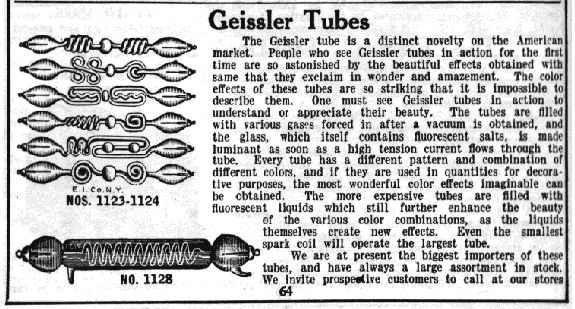
\includegraphics[width=\linewidth]{gfx/geissler1}
	\caption{An advertisement from the 1914 Electro Importing Catalog showing a variety of designs \cite{electro1914}.}
	\label{fig:geissler}
\end{figure}



\begin{figure}
    \centering
    \includegraphics[width=\linewidth]{gfx/dischargetubetemp1.png}
    \caption{TEMP Discharge tube. Make your own, it's not exactly complicated...}
    \label{fig:discharge}
\end{figure}

The next development was by Hittorf in 1869, who showed that the phosphorescence, or the phenomena responsible for said luminescence was intercepted by any solid, liquid, conductor or insulator placed between the negatively charged cathode and the tube walls \cite{hittorf:1869}. This identified the negatively charged cathode as the source of the phorphorescence, with the idea that this may be a gas which spreads uniformly like rays of light. Further to this, in 1876 Goldstein observed that with a large negatively biased terminal and similar blocking objects, well defined shadows could be obtained in the phosphorescence. One specific observation was that in contrast to light, sharp shadows were obtained even with blockers placed very close to the emitting cathode, implying that the emitted rays were not emitted evenly in all directions. This was the first work which referred to the rays as "Kathodenstrahlen", cathode rays.

In the 1970s, vacuum tubes began to make use of better vacuum pumping systems to achieve pressures of $0.1\si{\pascal}$--$0.005\si{\pascal}$ (down to 0.000005\% of atmospheric pressure, or 20000 times lower than the early Geissler tubes). With these high vacuum conditions, it was observed that the glass at the anode side of the tube would glow via fluorescence, rather than the entirety of the glass tube as in the Geissler tube. These high vacuum tubes are sometimes referred to as "Crookes tubes" due to the observations reported by William Crookes in 1879 \cite{crookes1879}. These observations included the consideration that the cathode ray may be composed of negatively charged particles being projected at a large velocity, and that there was a deflection at right angles when a magnetic field was present. While Crookes believed these particles to be "radiant matter", Hertz and Goldstein claimed they were "aether vibrations", or a form of electromagnetic waves \cite{thomson:1903}. In 1897, J. J. Thomson resolved this question with measurements of the particle mass, revealing that they had a mass around 1800 times smaller than that of the mass of a hydrogen atom \cite{thomson:1901}. This was achieved through application of a magnetic field at right angles to induce a circular path, such that measurement of the radius gains the effective mass of the particle, which became known as the electron. 

\subsection{Rectifying Diode}
In 1904, the electronic vacuum tube was invented which had pressures down to $10^{-9}$ atmospheres, $10^{-4}\si{\pascal}$. At pressures more than 50 times lower than that of Crookes tubes, there are so few gas molecules that there is no longer conduction via ionisation and instead electrons are injected into the vacuum via thermionic emission from a hot cathode. Thermionic emission was also known as the "Edison effect", due to experiments performed by Edison in 1883. One of the issues that Edison was facing with filament light bulbs at the time was that of the bulb darkening over time due to an accumulation of soot inside the glass. In an attempt to solve this problem, he inserted a metal electrode, hoping that the soot would be attracted to the electrode rather than that of the glass, then applied both a positive and negative bias \cite{nebeker:2009}. He noted that a current would flow when the plate was positively biased, but not when it was negative. This current also depended upon the filament temperature, however this predated the discovery of the electron and so Edison had no theory for why this may be happening and only noted his observations. He then filed the first patent for devices making use of this effect in 1884 \cite{edison:1884}. 

\begin{figure}
    \centering
    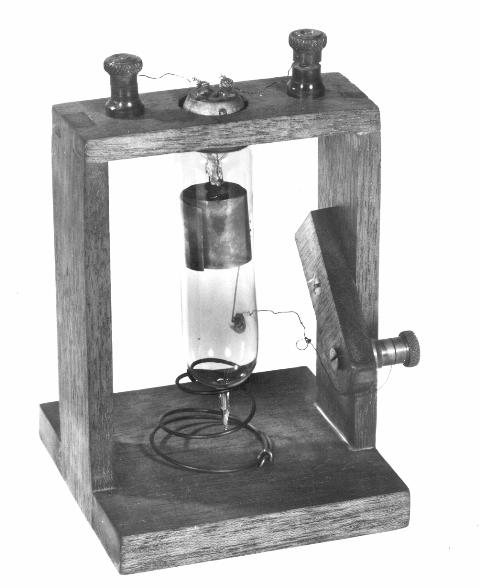
\includegraphics[width=0.6\linewidth]{gfx/fleming_diode.jpg}
    \caption{An early Fleming Diode, sourced from \cite{ethw:2008}.}
    \label{fig:fleming_diode}
\end{figure}

The initial invention of the vacuum diode is a contentious issue, as this was a device in the making around the world in various forms. However, it is generally accepted that the first invention of a practical vacuum tube device was in 1904 by J. A. Fleming. This device was a simple vacuum "diode" containing a hot electron emitting cathode and an anode, which only allowed for current to pass in one direction within a circuit \cite{fleming:1905}. This also went by the name of a "Fleming valve", and was initially built to be used as a detector for early radio receivers. By introducing a device that only allows for current to pass in one direction, Fleming was able to convert a weak alternating signal (current flowing in both directions at a certain frequency) into a direct current (current passing in one direction only) which could then feed into a telephone receiver for clear communication.%[Thomson1903 in books page 139 properties of the cathode rays for an excellent account of the history with direct sources, better than anything else I've found??] More to do, I like his line of writig even if it's a bit of a waste of time eh

\subsection{Triode}
The triode vacuum tube is a type of vacuum tube that consists of an electron emitter, known as a cathode, a control grid and an anode. It was invented in 1906 by Lee De Forest and marked a major milestone in the history of electronics.

\begin{figure}
    \centering
    
\includegraphics[width=0.4\linewidth]{gfx/Triode_symbol.png}
    \caption{A circuit-style diagram of a triode, with a curved cathode to indicate the flow of elctrons from the bottom to the top, passing through the "gate" grid.}
    \label{fig:triode_symbol}
\end{figure}

Before the invention of the triode, the rectifying diode was the primary electrical usage of vacuum tubes. These diodes only contain the cathode and anode. De Forest added a third element, the control grid, to the diode vacuum tube to create the triode vacuum tube. This is depicted in a typical circuit diagram in figure \ref{fig:triode_symbol}. The control grid allowed for the flow of electrons from the cathode to the anode to be controlled by a small electrical signal applied to the grid. This made it possible to use the triode as an amplifier, which is a device that increases the amplitude of an electrical signal. This was a major breakthrough in the field of electronics, as it made it possible to take weak electrical signals, such as radio or telegraph signals, and amplify them to a level which is audible for the listener when passed into a speaker.

The triode was initially only used as a detector of wireless signals, partly due to the residual air limiting device performance, but in 1912 several independent researchers recognised that the triode had massive potential for amplification purposes. This generalisation led to usages in a wide range of other applications, playing a critical role in the development of electronics. This paved the way for the invention of the semiconductor transistor, which replaced the original vacuum tube devices.

Generally, vacuum tubes found several applications in electronics:
\begin{itemize}
    \item Radio receivers: As well as diodes, grid controlled triodes were used to amplify weak radio signals, making them audible to the listener.
    \item Television sets: Early television sets used vacuum tubes to generate and amplify the video and audio signals that were displayed on the screen.
    \item Computers: The first generation of electronic computers relied on vacuum tubes to perform logical operations and store data.
    \item Amplifiers: Similar to radio receivers, audio amplifiers also used vacuum tubes to drive loudspeakers and produce audible sound.
    \item Oscilloscopes: The electrical signal to be measured can be applied to the grid of a vacuum tube, amplifying the input signal which is then used in a cathode ray tube to produce a visible display.
    \item Other communication systems: The telegraph and telephone networks widely used vacuum tubes to amplify and switch electrical signals.
\end{itemize}

\section{Silicon Transistors: Surpassing Vacuum Tube Technology}
The transistor, often considered the cornerstone of modern electronics, revolutionised the field of electronics by offering an alternative to the bulky and less efficient vacuum tubes. Its development marked the beginning of miniaturisation and enhanced performance of electronic devices, paving the way into the information age which we currently live in.

\subsection{Creation of the Transistor} 
The invention of the transistor in 1947 by John Bardeen, Walter Brattain, and William Shockley at Bell Laboratories was a major breakthrough that set the stage for the semiconductor era of electronics. The initial form of transistors was the point-contact transistor, a small, efficient, and more reliable alternative to the vacuum tube based diode. This discovery won the trio the Nobel Prize in Physics in 1956 and was the start of solid-state electronics, so named due to their ability to incorporate multiple electrical elements within a single solid piece of material. Instead of metal grids and electrodes separated by vacuum, the same effects could be achieved by changing the material properties of regions within semiconductors.

\subsection{Silicon} 
While the earliest transistors were made using germanium, silicon quickly became the material of choice due to its superior thermal stability and relative abundance due to methods of production such as the Czochralski method developed in 1915 (crystallising highly pure and large silicon ingots through the careful drawing of material from a molten state). Silicon transistors offered several advantages over vacuum tubes and germanium transistors, including lower power consumption, smaller size, greater reliability, and a longer lifespan. The ability of silicon to form a stable oxide layer (SiO2) was instrumental in the development of metal-oxide-semiconductor field-effect transistors (MOSFETs), which became the backbone of digital circuits, effectively replacing the vacuum triode.

\subsection{From Discrete to Integrated} 
The evolution of transistors led to the miniaturisation and integration of circuits. In 1958, Jack Kilby and Robert Noyce independently developed the integrated circuit (IC), which integrated multiple transistors and other components onto a single silicon chip. This innovation drastically reduced the size and cost of electronic devices and laid the foundation for the modern computer and electronics industry. Nowadays, it is highly normalised for ICs to be present in almost every device, with the internet of things (IoT) becoming an everyday standard where washing machines, fridges, and doorbells are now capable of sharing information with users over the internet. This is all thanks to IC chips, and the microscopic scale of modern transistors based on silicon.

\subsection{The Digital Revolution} 
The proliferation of silicon transistors fueled the digital revolution, starting the second generation of computers and exponentially improving upon the foundations laid by vacuum tubes. As transistor sizes shrank, the computing power of silicon-based chips surged, enabling the rise of personal computers, smartphones, and the digital world at large. This is commonly referred to with Moore's law, named after Gordon Moore, who in 1975 predicted that every two years the number of transistors in an IC will double. Despite regular challenges in recent decades, this has remained true from 1970 all the way into 2023, thanks in large part to the discovery of new device structures that are able to avoid the quantum limitations encountered by electronic devices which have a similar size to several layers of atoms. Silicon transistors have been instrumental in the advancement of modern technology, from microprocessors and memory chips to sensors and power management devices. 

%put a moore's law graph in here? but where from ffs? https://ourworldindata.org/moores-law goes to 2021, but I know "The highest transistor count in a consumer microprocessor is 134 billion transistors, in Apple's ARM-based dual-die M2 Ultra system on a chip, which is fabricated using TSMC's 5 nm semiconductor manufacturing process." this is twice the end of 2022 so.... what actually counts for this plot? should I scrape a bit of data and make my own? not too hard to do, but how do they differentiate between supercomputer cpu's (2.6 trillion cerebras as of 2020 7nm?>???) awkward problem, this doesn't matter that much, just nice to have

\subsection{Challenges and Competition with Silicon} 
Despite the remarkable success of silicon transistors, the relentless miniaturisation raises challenges such as increased leakage currents and heat generation. Innovations in transistor design such as FinFETs and Multi-Gate transistors have been developed to address these challenges, pushing the boundaries of silicon technology further. However these novel approaches are sill fundamentally limited by the silicon at the heart of such devices. Alternative materials have been the subject of intense study over the last few decades, with significantly superior material properties offering improvements in efficiency and miniaturisation of high power devices, to name two key areas of study. The climate crisis is ever looming, putting pressure on research to find new solutions for a world which is increasingly dependent upon IC chips. In particular, study is focused on using less power to achieve the same results, with natural benefits from a cost and performance perspective also arising as the cost of manufacturing these materials is reduced. Much as the old vacuum tubes are now considered to be dated, inefficient, and unreliable devices, perhaps silicon based technology will be viewed in a similar light in the decades ahead.

\subsection{Current Day}

\section{Beyond Silicon}
\subsection{Light Emitting Diodes (LED's)}
Light emitting diodes (LEDs) are based on p-i-n junctions that emit light when a forward voltage is applied. LEDs are widely used for illumination, displays, and optical communications, among other applications. While silicon-based LEDs are commonly used due to their low cost, LEDs based on other semiconductors such as gallium nitride (GaN) are vital to the production of white light, since the wider bandgap of GaN allows for the creation of blue LED's. The fabrication of GaN-based LEDs involves epitaxial growth of a thin GaN layer on a sapphire or silicon carbide substrate, followed by the formation of p-i-n junctions and metal contacts. These processes can be performed using techniques such as metalorganic chemical vapor deposition (MOCVD) and plasma-assisted molecular beam epitaxy (PAMBE).

\subsection{Extreme Conditions}
Silicon has been a widely used semiconductor for many years due to the combination of excellent electrical properties, a well-established fabrication process, and the availability of high-purity crystalline material. Silicon's abundance and the ability to produce high-quality, large single crystals through methods such as the Czochralski process have made it a readily available material for large-scale production. Silicon's stable oxide layer and low interface-state density have also enabled the development of efficient and reliable transistors, making it the preferred material for integrated circuits, microprocessors, and a variety of other electronic devices.

However, when silicon reaches its temperature limit of around 125--150\si{\degreeCelsius}, the mobility of charge carriers decreases, causing increased electrical resistance and reduced device performance. The diffusion of dopants can also occur, leading to changes in the doping profile and altering the electrical properties of the device. Additionally, high temperatures can cause thermal stress that can lead to mechanical failure. The temperature limit for semiconductor devices is determined by several factors, including the thermal expansion coefficient of the materials used, the thermal conductivity of the device, and the melting point of the metal contacts used to make electrical connections. 

Another limiting condition is electrical breakdown, which occurs when the electric field in the device reaches a critical value and causes a flow of current through the material. In the case of high power densities, the high electric fields can cause electrons to gain enough energy to generate electron-hole pairs through impact ionisation, leading to an avalanche effect and the formation of a conductive path. Ionising radiation can also have a detrimental effect on the performance and reliability of silicon devices due to the generation of electron-hole pairs, effectively altering the doping profile and causing increased leakage currents. Finally, at high frequencies, the mobility of charge carriers in silicon decreases due to increased scattering events and limited time available for carriers to move across the device. This results in higher resistive losses and reduced device performance at high frequencies. Parasitic capacitance due to device geometry and packaging can also cause significant delay and attenuation of high frequency signals.

Wide bandgap materials such as silicon carbide (SiC) and gallium nitride (GaN) have gained interest due to their ability to operate at high temperatures and voltages, offering an improved performance compared to silicon. The bandgap values of these materials are larger than silicon, with SiC having an estimated bandgap range of 2.2--3.3 eV and GaN having an estimated bandgap range of 3.2--3.4 eV. The correspondingly wider bandgap of these materials means that a higher energy of electron collisions is required to generate electron-hole pairs, leading to a higher breakdown voltage. Wide bandgap materials also offer higher electron saturation velocities and reduced switching losses compared to silicon, resulting in higher efficiency and faster switching speeds. These advantages make wide bandgap semiconductors promising candidates for next-generation power electronics and high-frequency applications.
\subsection{Solar Panels}
Solar panels work by converting sunlight into electrical energy through the use of semiconductors. Specifically, solar panels use a photovoltaic cell to capture sunlight and convert it into electricity. A photovoltaic cell is made up of two layers of silicon, one of which is doped with boron to create a layer with a positive charge (p-type) and the other is doped with phosphorous to create a negatively charged layer (n-type). When photons of sunlight hit the solar panel, the energy from the photons in the sunlight creates electron hole pairs within the silicon. 

The p-type and n-type layers of silicon in the photovoltaic cell create a built-in electric field that causes the photon-induced free electrons to flow from the n-type layer to the p-type layer, and vice versa for the holes generated by photon absorption. This flow of charge carriers (both electrons and holes) creates a flow of electrical current, such that when the photovoltaic cell is connected in a circuit, the resulting current can be used as a source of electrical power.
\subsection{High Power Electronics}

\section{Diamond}
Diamond is a unique material with exceptional physical and electronic properties. It is a form of carbon that is composed of a three-dimensional network of covalently bonded carbon atoms. Its structure is a face-centered cubic lattice, with each carbon atom bonded to four neighbouring carbon atoms.
\subsection{Material Properties}
One of the key electronic properties of diamond is its wide electronic bandgap, which makes it an excellent insulator. The bandgap of diamond is approximately 5.5 \si{\electronvolt}, which makes diamond an attractive material for electronic applications. Devices that successfully utilise diamond's wide bandgap will have a theoretically higher operating frequency and higher power levels than any of the more conventional semiconductors and even other wide bandgap semiconductors. The wide bandgap also makes diamond highly resistant to radiation damage, which makes it a strong contender in radiation detectors and other high energy applications where ionising radiation may cause issues in smaller bandgap materials.
\subsection{Current Applications}
One of the current applications of diamond in electronic devices is in the fabrication of high-performance field-effect transistors (FETs) and diodes. Diamond FETs offer superior performance compared to traditional silicon-based FETs, including higher current density, higher breakdown voltage, and faster switching speeds. Diamond diodes are also being developed for use in high-power rectifiers and detectors. Additionally, diamond is being investigated for use in radiation-hard electronics and quantum information processing.
\subsection{Future Applications}